\documentclass[tikz,border=8pt]{standalone}
\usepackage{lmodern}
\usetikzlibrary{arrows.meta,positioning,shapes.geometric}
\definecolor{ink}{HTML}{183B4E}
\definecolor{teal}{HTML}{168C8C}
\definecolor{gold}{HTML}{D9982F}
\definecolor{violet}{HTML}{7B61A8}
\definecolor{softblue}{HTML}{EAF4F6}
\definecolor{softgold}{HTML}{FFF4D8}
\begin{document}
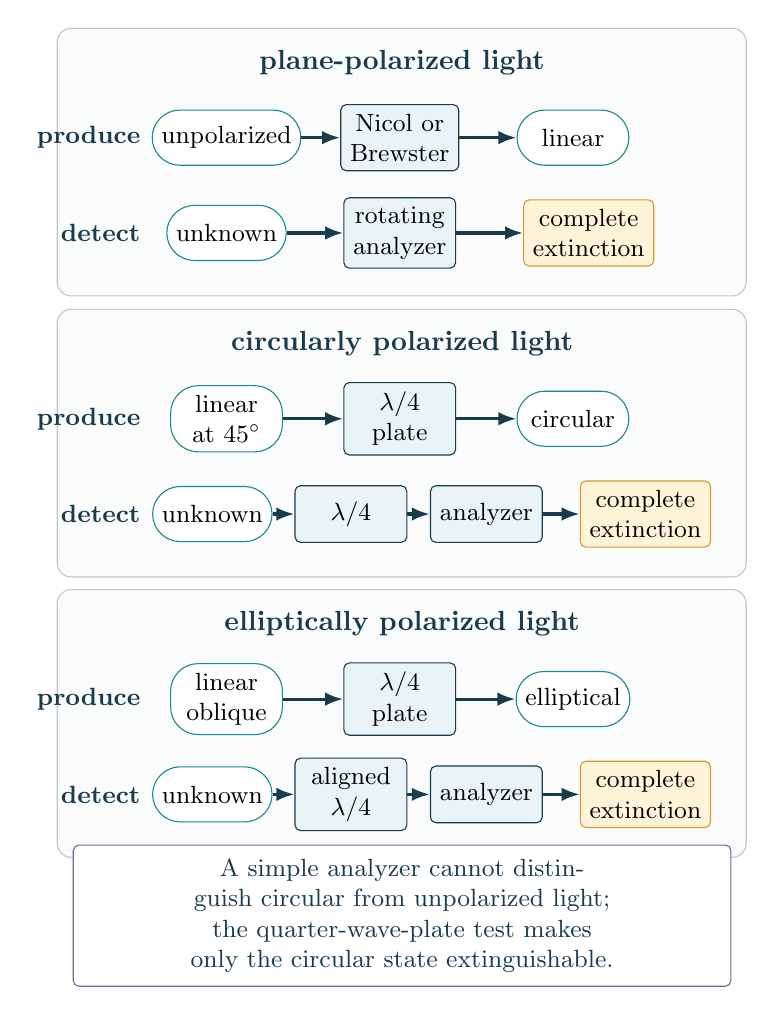
\begin{tikzpicture}[>=Latex,font=\sffamily]
  \tikzset{
    element/.style={draw=ink,fill=softblue,rounded corners=2pt,minimum width=1.42cm,minimum height=.72cm,align=center,font=\small},
    state/.style={draw=teal,fill=white,rounded corners=10pt,minimum width=1.42cm,minimum height=.70cm,align=center,font=\small},
    result/.style={draw=gold,fill=softgold,rounded corners=2pt,minimum width=1.56cm,minimum height=.72cm,align=center,font=\small},
    flow/.style={ink,line width=1.15pt,-{Latex[length=2.3mm]}}
  }

  % Linear card.
  \path[draw=ink!28,fill=ink!2,rounded corners=5pt] (-.1,7.15) rectangle (8.65,10.55);
  \node[text=ink,font=\bfseries] at (4.28,10.12) {plane-polarized light};
  \node[text=ink,anchor=east,font=\small\bfseries] at (1.08,9.16) {produce};
  \node[state] (Lu) at (2.05,9.16) {unpolarized};
  \node[element] (Lp) at (4.25,9.16) {Nicol or\\Brewster};
  \node[state] (Ll) at (6.45,9.16) {linear};
  \draw[flow] (Lu)--(Lp); \draw[flow] (Lp)--(Ll);
  \node[text=ink,anchor=east,font=\small\bfseries] at (1.08,7.95) {detect};
  \node[state] (Lx) at (2.05,7.95) {unknown};
  \node[element] (La) at (4.25,7.95) {rotating\\analyzer};
  \node[result] (Le) at (6.65,7.95) {complete\\extinction};
  \draw[flow] (Lx)--(La); \draw[flow] (La)--(Le);

  % Circular card.
  \path[draw=ink!28,fill=ink!2,rounded corners=5pt] (-.1,3.58) rectangle (8.65,6.98);
  \node[text=ink,font=\bfseries] at (4.28,6.55) {circularly polarized light};
  \node[text=ink,anchor=east,font=\small\bfseries] at (1.08,5.59) {produce};
  \node[state] (Cl) at (2.05,5.59) {linear\\at $45^\circ$};
  \node[element] (Cq) at (4.25,5.59) {$\lambda/4$\\plate};
  \node[state] (Cc) at (6.45,5.59) {circular};
  \draw[flow] (Cl)--(Cq); \draw[flow] (Cq)--(Cc);
  \node[text=ink,anchor=east,font=\small\bfseries] at (1.08,4.38) {detect};
  \node[state] (Cx) at (1.87,4.38) {unknown};
  \node[element] (Cdq) at (3.63,4.38) {$\lambda/4$};
  \node[element] (Ca) at (5.35,4.38) {analyzer};
  \node[result] (Ce) at (7.37,4.38) {complete\\extinction};
  \draw[flow] (Cx)--(Cdq); \draw[flow] (Cdq)--(Ca); \draw[flow] (Ca)--(Ce);

  % Elliptical card.
  \path[draw=ink!28,fill=ink!2,rounded corners=5pt] (-.1,.02) rectangle (8.65,3.42);
  \node[text=ink,font=\bfseries] at (4.28,2.99) {elliptically polarized light};
  \node[text=ink,anchor=east,font=\small\bfseries] at (1.08,2.03) {produce};
  \node[state] (El) at (2.05,2.03) {linear\\oblique};
  \node[element] (Eq) at (4.25,2.03) {$\lambda/4$\\plate};
  \node[state] (Ee) at (6.45,2.03) {elliptical};
  \draw[flow] (El)--(Eq); \draw[flow] (Eq)--(Ee);
  \node[text=ink,anchor=east,font=\small\bfseries] at (1.08,.82) {detect};
  \node[state] (Ex) at (1.87,.82) {unknown};
  \node[element] (Edq) at (3.63,.82) {aligned\\$\lambda/4$};
  \node[element] (Ea) at (5.35,.82) {analyzer};
  \node[result] (Eex) at (7.37,.82) {complete\\extinction};
  \draw[flow] (Ex)--(Edq); \draw[flow] (Edq)--(Ea); \draw[flow] (Ea)--(Eex);

  \node[draw=violet,fill=white,rounded corners=2pt,align=center,text width=8.0cm,inner sep=5pt,text=ink,font=\small]
    at (4.28,-.72)
    {A simple analyzer cannot distinguish circular from unpolarized light;\\the quarter-wave-plate test makes only the circular state extinguishable.};
\end{tikzpicture}
\end{document}
